% Substrate inheritance / provenance overview.
% Designed for full text-width.
\begin{figure}[t]
\centering
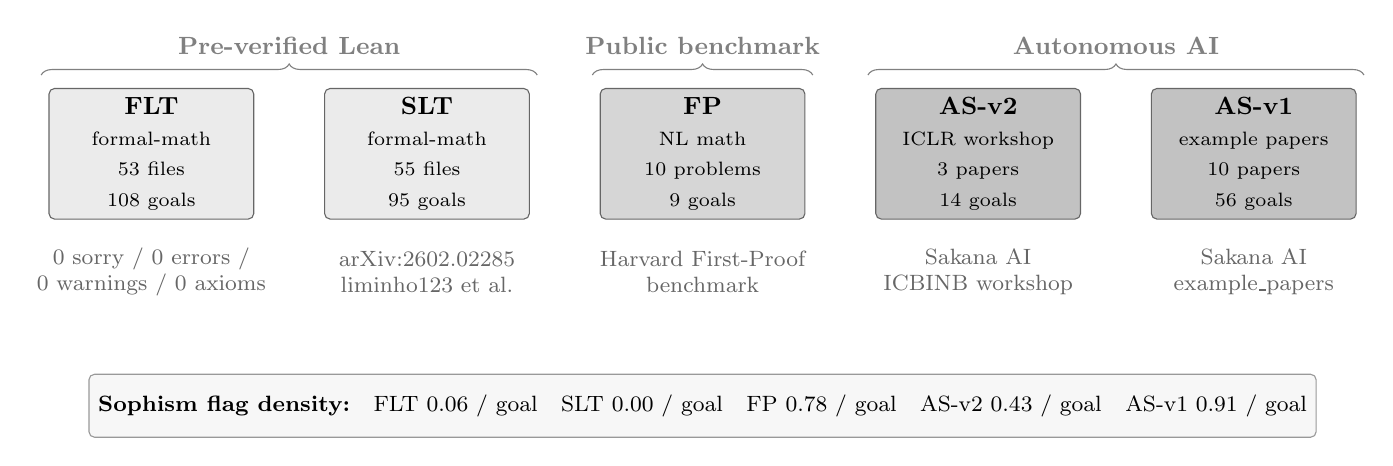
\begin{tikzpicture}[
  font=\small,
  substrate/.style={
    rectangle, rounded corners=2pt, draw=black!60,
    minimum width=2.6cm, minimum height=1.6cm, align=center
  },
  formal/.style={substrate, fill=black!8},
  empirical/.style={substrate, fill=black!16},
  ai/.style={substrate, fill=black!24},
  brace/.style={decorate, decoration={brace, amplitude=4pt}, black!50},
  flow/.style={-{Latex[length=2mm]}, black!70, line width=0.5pt, dashed},
]

% Five substrates in a row
\node[formal] (flt) at (-7.0, 0)
  {\textbf{FLT}\\\scriptsize formal-math\\\scriptsize 53 files\\\scriptsize 108 goals};
\node[formal] (slt) at (-3.5, 0)
  {\textbf{SLT}\\\scriptsize formal-math\\\scriptsize 55 files\\\scriptsize 95 goals};
\node[empirical] (fp) at (0, 0)
  {\textbf{FP}\\\scriptsize NL math\\\scriptsize 10 problems\\\scriptsize 9 goals};
\node[ai] (asv2) at (3.5, 0)
  {\textbf{AS-v2}\\\scriptsize ICLR workshop\\\scriptsize 3 papers\\\scriptsize 14 goals};
\node[ai] (asv1) at (7.0, 0)
  {\textbf{AS-v1}\\\scriptsize example papers\\\scriptsize 10 papers\\\scriptsize 56 goals};

% Group labels (above)
\draw[brace] (-8.4, 1.0) -- (-2.1, 1.0)
  node[midway, above=4pt, font=\small\bfseries] {Pre-verified Lean};
\draw[brace] (-1.4, 1.0) -- (1.4, 1.0)
  node[midway, above=4pt, font=\small\bfseries] {Public benchmark};
\draw[brace] (2.1, 1.0) -- (8.4, 1.0)
  node[midway, above=4pt, font=\small\bfseries] {Autonomous AI};

% Provenance row
\node[font=\footnotesize, black!60, align=center] at (-7.0, -1.5)
  {0 sorry / 0 errors / \\ 0 warnings / 0 axioms};
\node[font=\footnotesize, black!60, align=center] at (-3.5, -1.5)
  {arXiv:2602.02285 \\ liminho123 et al.};
\node[font=\footnotesize, black!60, align=center] at (0, -1.5)
  {Harvard First-Proof \\ benchmark};
\node[font=\footnotesize, black!60, align=center] at (3.5, -1.5)
  {Sakana AI \\ ICBINB workshop};
\node[font=\footnotesize, black!60, align=center] at (7.0, -1.5)
  {Sakana AI \\ example\_papers};

% Discriminative axis annotation (below)
\node[align=center, font=\footnotesize, draw=black!40, fill=black!3,
      rounded corners=2pt, minimum width=14cm, minimum height=0.8cm] at (0, -3.2)
  {\textbf{Sophism flag density:}\quad
   FLT 0.06 / goal\quad SLT 0.00 / goal\quad
   FP 0.78 / goal\quad AS-v2 0.43 / goal\quad AS-v1 0.91 / goal};

\end{tikzpicture}
\caption{Substrate inheritance and provenance. The five substrates span three
qualitatively different artifact types: pre-verified clean Lean
formalizations (FLT, SLT), a public natural-language mathematical research
benchmark (FP), and autonomous-AI-generated paper artifacts (AS-v2, AS-v1).
Goal-counts are the dataset's per-substrate population. The sophism-flag
density annotated at the bottom is the headline discriminative result.}
\label{fig:substrate_inheritance}
\end{figure}
